\documentclass[10pt,a4paper]{article} % tamaño de letra y tipo de papel
\usepackage[utf8]{inputenc}
\usepackage[spanish]{babel} % paquete para que reconozca ñ y tildes
\usepackage{amsmath}
\usepackage{amsfonts}
\usepackage{amssymb}
\usepackage{graphicx} % paquete para incluir imagenes
\usepackage[margin=1in,bottom=1in]{geometry}
\usepackage{hyperref} % paquete para tener marcadores en el pdf
\author{Ulloa Daniel}
\begin{document}

\begin{titlepage}
	\hbox{
		\hspace*{0.15\textwidth} % Espacio desde el margen izquierdo
		\rule{1pt}{\textheight} % Linea decorativa
		\hspace*{0.05\textwidth} % Espacio entre la linea y el texto
		\parbox[b]{0.75\textwidth}{ % Caja que restringe el espacio que puede ocupar el texto
			{\noindent\Huge\bfseries Informe de Laboratorio } % Titulo
			\\ 
			[2\baselineskip] 
			{\large \textbf{Tema:} Oscilador con Resistencia Negativa} % Tema
			\\[4\baselineskip]
            {\large \textbf{Cátedra:} Teoría de Circuitos \textsc{II}} % Catedra
            \\[1\baselineskip]
            {\large \textbf{Año:} 2019} % Año
			\\[1\baselineskip]
            {\large \textit{\textbf{Docentes:} % Docentes
                \textnormal{Ing. Costa}, Nicolás. 
                \textnormal{Aux. Consiglio}, Dante}
            }
			\\[1\baselineskip]
            {\large \textit{\textbf{Alumnos:} % Alumnos
                \textnormal{Rodriguez}, Ana Victoria. 
                \textnormal{Ulloa}, Daniel Alejandro}
            }
            \\[6\baselineskip]
            {\large \textbf{Fecha de Entrega:} 11/09/2019}
			\par %Para que el logo aparezca al pie
			\vspace{0.35\textheight} % Ubicacion de la caja desde el margen superior
            \center{
\includegraphics[width=250px]{logo2.png}}
            \\[1\baselineskip]
	}}
\end{titlepage}
\tableofcontents
\newpage
\section{Introducción}

\section{Objetivos}
\begin{itemize}
    \item Modelar e interpretar el Circuito
    \item Obtener la respuesta temporal de la tensión de salida y graficarla en Mathematica
    \item Realizar un barrido paramétrico sobre la resistencia $R_B$ y observar las diferentes respuestas.
\end{itemize}
\section{Modelado Matemático}
El circuito a modelar se muestra a continuación %sopenca
\begin{center}
%    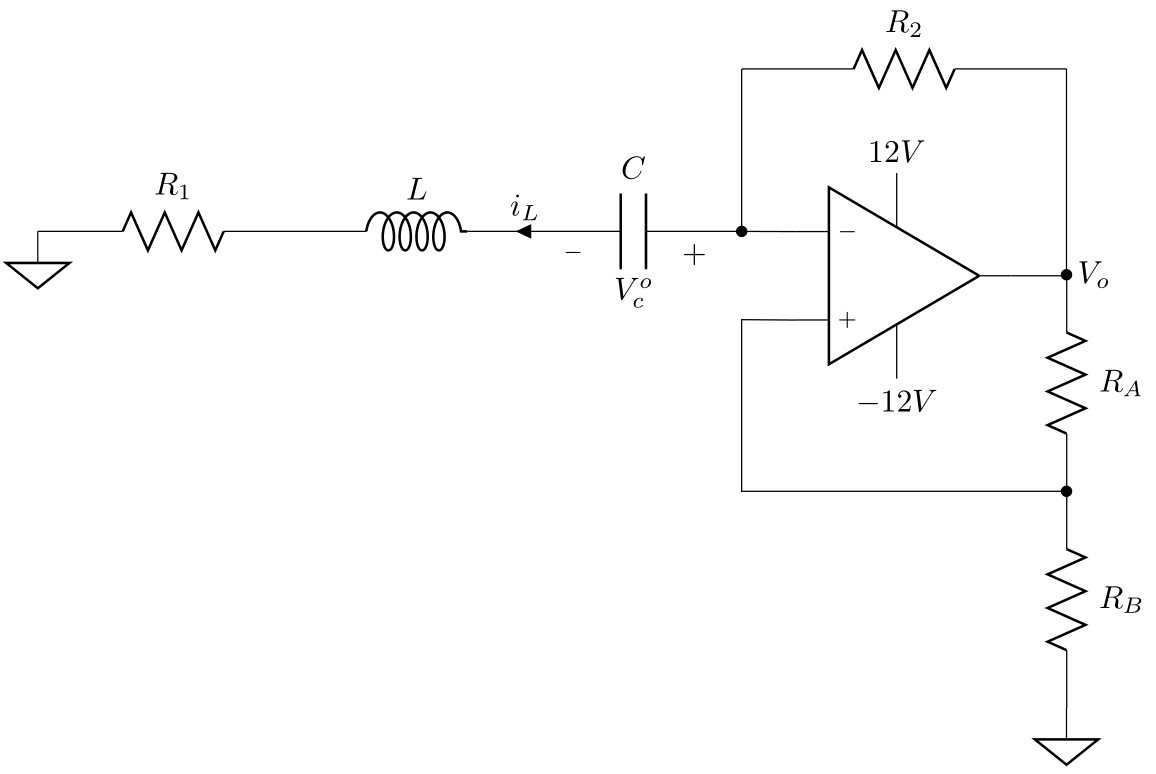
\includegraphics[width=300px]{circuito}
\end{center} 
Se consideró el amplificador operacional ideal y se analizó el nodo $V_{n}$.
Se tiene dos corrientes en $V_{n}$, la correspondiente al RLC y la que pasa por la resistencia R2. \\
\begin{equation}
i(t)=i_{r2}(t)
\end{equation}
Sabiendo que la corriente que pasa por el RLC es la del capacitor dado a que es el elemento con condiciones iniciales, esta es igual a 
\begin{equation}
i(t)=C_{1}*V_{c}'(t)
\end{equation}
y la corriente que pasa por la resistencia R2 
\begin{equation}
i_{r2}(t)=\frac{V_{n}(t)-V_{o}(t)}{R2}
\end{equation}
Donde las tensiones $V_{n}(t)$ y $V_{p}(t)$ son iguales al considerar que el amplificador operacional es ideal, y su vez , que  $V_{p}$ es la tensión de un divisor de tensión formado por las resistencias Ra y Rb y la tensión de salida  $V_{o}(t)$. 

\begin{equation}
V_{p}(t)=\frac{\text{Rb}* V_{o}(t)}{\text{Ra}+\text{Rb}}
\end{equation}
De esta manera se obtiene la primera ecuación de nuestro sistema, a la cual se le aplicó la transformada de Laplace, obteniendo 
\begin{equation}
eq1=C{1}* (s V_{c}(s)-V_{c}(t))+\frac{\text{Ra}* V_{o}(s)}{\text{R2} \text{Ra}+\text{R2} \text{Rb}}
\end{equation}
Para la segunda ecuación se recorrio la malla que contiene a los componentes R1,R2, C, y L, cuya suma de las tensiones es igual a la tensión en la salida. 
\begin{equation}
\ V_{o}(t)=\ V_{c}(t)+ V_{l}(t)+ V_{r}(t)
\end{equation}
\begin{equation}
V_{o}(t)=C*L*V_{c}''(t)+ C*(\text{R1}+\text{R2})*V_{o}'(t)+V_{c}(t)
\end{equation}
Nuevamente se aplico la transformada de Laplace, obtiendo la segunda ecuación
\begin{equation}
eq2 = V_{c}(s) - V_{o}(s) + C1*(R1 + R2)*(s*V_{c}(t) - V_{0}(t)) + 
L1*C1*(s^{2}*V_{c}(t) - s*V_{0}(t))
\end{equation}
\section{Respuesta Temporal}
\section{Barrido Paramétrico}
\section{Conclusión}
\end{document} 


